% Лекции Сергея Борисовича Стечкина
% Внесены исправления В.В.Арестова, версия 06.07.2009
% Внесены исправления Н.И.Черныха, версия 24.07.2009
% Внесена грамматическая и ТеХ-правка М.Дейкаловой, версия 05.08.09

 %%%%%%%%%%%%%%%%%%%%%%%%%%%%%
 \chapter{Приближение истокообразно представимых функций}
  %%{Лекция 18.}



 \section{Приближение  функций в пространстве  $L_{2\pi}$
 %\\ тригонометрическими полиномами
 }

Рассмотрим вначале  наилучшее приближение функций в пространстве $L= L_{2\pi},$
наделенном нормой
$$
\|f\|_L=\frac{1}{\pi}\int_{0}^{{2\pi}}|f(t)|dt,
$$ тригонометрическими
 полиномами
 $$
 t_{n-1}(x)=\frac{\alpha_0}{2}+\sum\limits_{k=1}^{n-1} (\alpha_k\cos
 kx+\beta_k \sin kx)
 $$
 порядка $n-1,$~ $n\ge 1.$



 \begin{teo}\label{approx_L} \it{ Для функций  $f\in L_{2\pi}$ справедливы
 следующие два утверждения:

 $1)$ Если для тригонометрического полинома $t_{n-1}^{{*}}$ функция, равная знаку разности
 $R=f-t_{n-1}^{{*}},$ ортогональна пространству ${\cal T}_{n-1}:$
 \begin{equation}\label{f18-1}
 \sign R \perp {t_{n-1}}\qquad \forall\  {t_{n-1}\in\mathcal{T}_{n-1}}, %\eqno(1)
  \end{equation}
 то $t_{n-1}^*$  --  полином наилучшего приближения функции $f$ в $L_{2\pi}$.


 $2)$ Если  $t_{n-1}^{{*}}$ -- полином наилучшего приближения функции $f$ и разность
 $f-t_{n-1}^{{*}}$ почти всюду отлична от нуля, то обязательно выполняется
 условие~$(\ref{f18-1}).$}
 \end{teo}

 В конце лекции 9 говорилось о возможном выводе подобного
 результата для приближения в $L(Q)$ из приведенного там
 доказательства критерия элемента наилучшего приближения в
 $L^p(Q).$ Ниже приводится полное доказательство для
 рассматриваемого частного случая.


 \begin{proof}
 %Д о к а з а  т е л ь с т в о\ \  л е м м ы.
 Предположим, что для
 тригонометрического полинома $t_{n-1}^{{*}}$ выполняется свойство~$(\ref{f18-1}),$
 т.\,е.  функция $\sign R$
 ортогональна  любому полиному порядка $n-1.$ Тогда  для любого полинома
 {$t_{n-1}\in {\cal T}_{n-1}$}
 $$
 \|f-t_{n-1}^{{*}}\|_L=\frac{1}{\pi}\int_0^{2\pi} |f(x)-t_{n-1}^{{*}}(x)|\, dx=
 \frac{1}{\pi}\int_0^{2\pi} (f(x)-t_{n-1}^{{*}}(x))\ \sign R(x)\, dx=
 $$
 $$
 =\frac{1}{\pi}\int_0^{2\pi} ((f(x)-{t}_{n-1}(x))+({t}_{n-1}(x)-t_{n-1}^{{*}}(x)))\
 \sign R(x)\, dx=
 $$
 $$
 =\frac{1}{\pi}\int_0^{2\pi} (f(x)-{t}_{n-1}(x))\ \sign R(x)\, dx\le
 \frac{1}{\pi}\int_0^{2\pi} |f(x)-{t}_{n-1}(x)|\, dx=\|f-{t}_{n-1}\|_L.
 $$
Следовательно, $t_{n-1}^{{*}}$ -- наилучший полином для функции $f$ в {$L_{2\pi}$
среди полиномов из $\mathcal{T}_{n-1}$.}

Предположим теперь, что $t_{n-1}^{{*}}$ -- полином наилучшего
приближения функции $f$ и почти всюду $t_{n-1}^{{*}}\ne f.$ Для произвольного полинома
${t}_{n-1}$ порядка $n-1$ определим функцию
$$
\Phi(\lambda)=\|f-(t_{n-1}^{{*}}-\lambda {t}_{n-1})\|_L=\frac{1}{\pi}\int_{0}^{2\pi}|f(x)
-t_{n-1}^{{*}}(x)+\lambda {t}_{n-1}(x))|\, dx
$$
вещественного переменного $\lambda.$
Убедимся, что функция $\Phi$ дифференцируема в точке $\lambda=0$ и
вычислим производную $\Phi'(0).$

Для вещественных чисел $a\ne 0$ и $b$ функция $\phi(\lambda)=|a+\lambda b|$ переменного
$\lambda$  дифференцируема в точке $\lambda=0$ и $\phi'(0)=b\ \sign a.$ Кроме того,
имеет место неравенство
$$
\left|\frac{|a+\lambda b|-|a|}{\lambda}\right|\le |b|,\qquad \lambda\ne 0.
$$
Применяя теорему Лебега о мажорантной сходимости, теперь нетрудно убедиться, что функция
$\Phi$ дифференцируема  в точке $\lambda=0$ и
$$
\Phi'(0)=\frac{1}{\pi}\int_{0}^{2\pi}\  {t}_{n-1}(x)\ \sign (f(x)-t_{n-1}^{{*}}(x))\,dx.
$$
В силу экстремальности полинома $t_{n-1}^{{*}}$ точка $\lambda=0$ является точкой минимума
функции~$\Phi;$ поэтому  $\Phi'(0)=0$ и мы пришли к свойству~$(\ref{f18-1}).$
Теорема~\ref{f18-1} доказана.
\end{proof}

 Заметим, что если выполняется условие~(\ref{f18-1}), то
 $$
 E_{n-1}(f)_L=\frac{1}{\pi}\int_0^{2\pi} (f(x)-t_{n-1}^{{*}}(x))\ \sign R(x)\, dx=
 \frac{1}{\pi}\int_0^{2\pi} f(x)\ \sign R(x)\, dx
 $$
и, окончательно,
 \begin{equation}\label{f18-2}
 E_{n-1}(f)_L=\frac{1}{\pi}\int_0^{2\pi} f (x)h^*(x)\, dx,%\eqno(2)
 \end{equation}
где $h^*=\sign R;$ при этом функция $h^*$ обладает свойствами
$\|h^*\|_{{L^\infty}}\le 1$ и $h^*\perp {t}_{n-1}$ для любого полинома
$t_{n-1}.$



 \begin{teo} %%% Теорема.
 Пусть $f\in L_{2\pi}.$ Тогда для любой функции {$h\in L_{2\pi}^\infty$} со свойствами
 $$
 \|h\|_{{L^\infty}}\le 1\quad \textit{и}\quad h\perp
 {t}_{n-1}\qquad \forall\ {t}_{n-1}
 $$
 выполняется неравенство
  \begin{equation}\label{f18-3}
 E_{n-1}(f)_L\ge \frac{1}{\pi}\int_0^{2\pi} f(x) h(x)\, dx.%\eqno(3)
  \end{equation}
 \end{teo}

 \begin{proof} %%% Доказательство.
 Пусть $t_{n-1}^*$ -- полином наилучшего приближения функции $f$ в $L.$
 В силу ортогональности функции  $h$ полиномам порядка $n-1$
 $$
 \frac{1}{\pi}\int_0^{2\pi} f(x)h(x)\, dx=\frac{1}{\pi}\int_0^{2\pi} (f(x)-t_{n-1}^*(x))h(x)\,dx\le
 \frac{1}{\pi}\int_0^{2\pi} |f(x)-t_{n-1}^*(x)|\,dx=E_{n-1}(f)_L.
 $$
  Теорема доказана.
 \end{proof}

\setcounter{corollary}{0}
\begin{corollary}
Предположим, что  $t_{n-1}^*$ -- полином наилучшего в $L_{2\pi}$
приближения  для функции $f$ и
функция  $h^*=\sign (f-t_{n-1}^*)$ удовлетворяет  условию~$(\ref{f18-1})$ $($к примеру,
разность $f-t_{n-1}^*$ не равна нулю почти всюду$).$ Тогда
 $$
 E_{n-1}(f)_L=\frac{1}{\pi}\int_0^{2\pi} f(x)h^*(x)\,dx=
 $$
 $$=\max \left\{\frac{1}{\pi}\int_0^{2\pi} f(x)h(x)\,dx:\
 h\in {L_{2\pi}^\infty},\ \|h\|_{{L^\infty}}\le 1;\ h\perp {t_{n-1}}\
 \forall\ {t_{n-1}}\in {\cal T}_{n-1}\right\}.
 $$
\end{corollary}

\begin{corollary}  Если полином {$t_{n-1}^*$} таков, что  разность {$f-t_{n-1}^*$} почти всюду
отлична от нуля и функция $h^{{*}}=\sign (f-t_{n-1}^{{*}}) $ ортогональна
пространству полиномов порядка $n-1,$ то {$t_{n-1}^*$} --
полином наилучшего приближения в $L_{2\pi}$ для функции $f,$ и неравенство
{\eqref{f18-3}} на функции $h^{{*}}$ и только на этой функции обращается в
равенство.
\end{corollary}

\ \

Любая функция $h$ {из $L_{2\pi}^\infty$} со свойствами
$$
\|h\|_{{L^\infty}}\le 1\quad \text{и}\quad h\perp t_{n-1}\qquad \forall\
t_{n-1}\in {\cal T}_{n-1}
$$
дает в силу {\eqref{f18-3}} для величины $E_{n-1}(f)_L$ оценку снизу.
 Выберем специальным образом функцию  $h.$ Предположим, что  $h$ имеет период  $\omega=\dfrac{2\pi}{n}$
 и $\ds\int_{-\pi}^{\pi} h(x)\, dx=0.$ Тогда ряд Фурье такой функции имеет вид
  $$
 h(x) \sim \sum\limits_{k=1}^{\infty} \alpha_{nk}\cos nkx+\beta_{nk}\sin nkx,
 $$
 т.\,е. у функции $h$ могут быть  отличны от нуля только коэффициенты
 Фурье, номера которых кратны числу $n.$
 В частности, выполняется свойство
 $$
 h\perp {t}_{n-1}\qquad \forall\  {t}_{n-1}.
 $$
 Поэтому в качестве $h$ в {\eqref{f18-3}}
 можно взять любую такую функцию (удовлетворяющую, помимо того, условию
 {$\|h\|_{L^\infty}\le 1$}).


 Возьмем функцию $h(x)=\sign \sin(nx+\alpha).$ Эта функция обладает
 всеми перечисленными свойствами: ее период
  $\omega$ равен $\dfrac{2\pi}{n},$~
 $ \dfrac{1}{\pi}\displaystyle\int_{-\pi}^{\pi} h(x)\, dx=0$ и {$\|h\|_{L^\infty}\le 1.$}
 Поэтому
  \begin{equation}\label{f18-4}
 E_{n-1}(f)_L\ge \frac{1}{\pi}\int_{-\pi}^{\pi} f(x)\, \sign\sin(nx+\alpha)\, dx\qquad
 \forall\ \alpha.%\eqno(4)
  \end{equation}
 Рассмотрим случаи $\alpha=0$ и $\alpha=\dfrac{\pi}{2}.$ Хорошо известно разложение
 $$
 \sign \sin x=\frac{4}{\pi}\sum\limits_{k=0}^{\infty}\frac{\sin
 (2k+1)x}{2k+1}.
 $$
Следовательно,
 %\addtocounter{equation}{1}
 \refstepcounter{equation}\label{f18-5}
 $$
 \sign \sin nx=\frac{4}{\pi}\sum\limits_{k=0}^{\infty}\frac{\sin
 (2k+1)nx}{2k+1}.\eqno(\theequation')
 $$
 Аналогично,
 $$
 \sign \cos x=\sign \sin\left( x+\frac{\pi}{2}\right)
 =\frac{4}{\pi}\sum\limits_{k=0}^{\infty}\frac{(-1)^k\cos
 (2k+1)x}{2k+1},
 $$
 $$
 \sign \cos nx=\frac{4}{\pi}\sum\limits_{k=0}^{\infty}
 \frac{(-1)^k\cos (2k+1)nx}{2k+1}.\eqno(\theequation'')
 $$
 В силу {\eqref{f18-4}}  для любой функции $f\in L$ справедливы
 $\Big($получаемые соответственно, при $\alpha=0$ и $\alpha=\dfrac{\pi}{2}\Big)$ оценки
 \begin{equation}\label{f18-6}
 E_{n-1}(f)_L\ge \frac{4}{\pi}\sum\limits_{k=0}^{\infty}
 \frac{b_{(2k+1)n}}{2k+1}, %\eqno(6)
 \end{equation}
 \begin{equation}\label{f18-7}
 E_{n-1}(f)_L\ge \frac{4}{\pi}\sum\limits_{k=0}^{\infty}
 \frac{(-1)^k a_{(2k+1)n}}{2k+1}, %\eqno(7)
 \end{equation}
 где $a_{(2k+1)n}$ и $b_{(2k+1)n}$ -- соответствующие индексам коэффициенты Фурье
  функции $f.$
    Заметим, что если $\alpha=\pi,$
 то $h(x)=-\sign \sin nx,$ если $\alpha=\dfrac{3}{2}\,\pi,$
 то $h(x)=-\sign\cos nx,$ и получим аналогичные оценки
 $$
 E_{n-1}(f)_{L}\ge
 -\frac{4}{\pi}\sum\limits_{k=0}^{\infty}\frac{b_{(2k+1)n}}{2k+1},
 \eqno(\ref{f18-6}')
 $$
 $$
 E_{n-1}(f)_{L}\ge
 -\frac{4}{\pi}\sum\limits_{k=0}^{\infty}\frac{(-1)^k a_{(2k+1)n}}{2k+1}.
 \eqno(\ref{f18-7}')
 $$

 Возникает вопрос, когда последние четыре оценки обращаются в равенство?
 Пусть $t_{n-1}^*$ -- полином наилучшего приближения функции $f.$
 Будем исходить из того, что   почти для всех  точек $x\in(-\pi,\pi)$ выполняется свойство $f(x)-t_{n-1}^*(x)\ne 0.$
 Равенство в {\eqref{f18-6}} возможно только в том случае, когда (почти всюду)
 \begin{equation}\label{f18-8}
 \sign(f-t_{n-1}^*)=\sign\sin nx; %\eqno(8)
 \end{equation}
 равенство в {\eqref{f18-7}} может быть, только если
 \begin{equation}\label{f18-9}
 \sign(f-t_{n-1}^*)=\sign\cos nx. %\eqno(9)
 \end{equation}
 Аналогично, равенство в~{$(\ref{f18-6}')$ и~$(\ref{f18-7}')$} будет, когда, соответственно,
 $$
 \sign(f-t_{n-1}^*)=-\sign\sin nx, \eqno(\ref{f18-8}')
 $$
 $$
 \sign(f-t_{n-1}^*)=-\sign\cos nx. \eqno(\ref{f18-9}')
 $$


 Предположим, что функция $f$ непрерывна на интервале $(-\pi,\pi).$
 Тогда {\eqref{f18-9} и~$(\ref{f18-9}')$} означают, что разность
 $f-t_{n-1}^*$ меняет знак в тех и только тех точках, где $\cos nx$
 обращается в нуль, и, значит, $t_{n-1}^*$ интерполирует $f$
 в нулях $\cos nx;$ аналогично,~{\eqref{f18-8} и~$(\ref{f18-8}')$}
 влекут, что $t_{n-1}^*$ интерполирует $f$ в нулях $\sin nx.$
 Эти условия интерполяции -- необходимые условия справедливости
 (для непрерывной функции) равенств в~{\eqref{f18-7}, $(\ref{f18-7}')$,
 \eqref{f18-6}, $(\ref{f18-6}')$,}
 соответственно. Однако в некоторых ситуациях они являются и  достаточными.
  Действительно, если полином $t_{n-1}$ интерполирует функцию $f,$ к примеру, {только}
 в нулях $\cos nx$ и разность $f-t_{n-1}$
 меняет знак в этих нулях и нигде больше, то в~{\eqref{f18-7}
  или~$(\ref{f18-7}')$}, соответственно,
 имеет место равенство и {$t_{n-1}^*$}
 является наилучшим полиномом для $f$ {в $L_{2\pi}$.} {В этих ситуациях}
 $$
 E_{n-1}(f)_L=\frac{4}{\pi}\left|\sum\limits_{k=0}^{\infty}
 \frac{b_{(2k+1)n}}{2k+1}\right|, \eqno(\ref{f18-6}'')
 $$
  $$
 E_{n-1}(f)_L=\frac{4}{\pi}\left|\sum\limits_{k=0}^{\infty}
 \frac{(-1)^k a_{(2k+1)n}}{2k+1}\right|.\eqno(\ref{f18-7}'')
 $$

 Таким образом, мы получили способ нахождения
 наилучшего полинома в $L_{2\pi}$ для $f\in C_{2\pi}$:
 выбираем $h(x)=\sign \sin nx,$ если $f$ -- нечетная, $h(x)=\sign \cos nx,$
 если $f$ -- четная (для других случаев следует рассмотреть функцию
 $\sign \sin (nx+\alpha)$ и попытаться подобрать соответствующим образом значение параметра
 $\alpha$). Затем строим полином, который
 интерполирует $f$ в нулях, соответственно, $\sin nx$ или $\cos nx$
 и проверяем знаки разности. Если они удовлетворяют
 соответствующим условиям~{\eqref{f18-8}, $(\ref{f18-8}'),$ \eqref{f18-9} или~$(\ref{f18-9}')$,}
 то наилучший полином построен. Так что задача построения
 наилучшего полинома в $L_{2\pi}$
 сводится к проверке знака разности $f-t_{n-1}^*.$
 Если знаки не проверять, то~{\eqref{f18-7}, $(\ref{f18-7}')$ и~\eqref{f18-6}
 или~$(\ref{f18-6}')$}
 дают оценку для $E_{n-1}(f)_L$ снизу.


 \section{Приближение классов функций в ${C}_{2\pi}$}

 Пусть  $K\in L_{2\pi};$ функцию $K$ будем называть  суммируемым  ядром.
 Рассмотрим класс функций $\G M=\G M_K,$  истокообразно представимых при помощи
 этого ядра, т.\,е. класс  функций вида
 \begin{equation}\label{f18-10}
 f(x)=c+\frac{1}{\pi}\int_0^{2\pi} K(t)\varphi(x+t)\,dt, %\eqno(10)
 \end{equation}
 где  $\varphi$ -- произвольная $2\pi$-периодическая функция из пространства
 {$L^\infty=L_{2\pi}^{\infty}$}
 со свойством $\|\varphi\|_{{L^\infty}}\le 1,$ а $c=c(f)$ -- вещественная константа.
 Функции из класса $\G M$ будут непрерывными $2\pi$-периодическими. Каждую
  функцию $f\in \G M$
  наилучшим образом приблизим тригонометрическими
 полиномами в $C_{2\pi}$ и возьмем
 $$
 \sup_{f\in \G M} \min_{t_{n-1}}\|f-t_{n-1}\|_C=E_{n-1}(\G M_K)_C;
 $$
 эту величину называют наилучшим приближением класса $\G M$
 в пространстве $C_{2\pi}$ множеством
 тригонометрических полиномов порядка $n-1$.

 Для любого тригонометрического полинома {$\widetilde{t}_{n-1}$}  функция
 $$
 t_{n-1}(x)=c+ \frac{1}{\pi}\int_0^{2\pi} \-{\widetilde{t}_{n-1}(t)} \varphi(x+t)\, dt
 $$
также является тригонометрическим полиномом  порядка $n-1$, и для него при
$c=c(f)$ имеем
 $$
 |f(x)-t_{n-1}(x)|=\left| \frac{1}{\pi}\int_0^{2\pi} \{ K(t)-{\widetilde{t}_{n-1}(t)}\}
 \varphi(x+t)\, dt \right|\le \frac{1}{\pi}\int_0^{2\pi} | K(t)-{\widetilde{t}_{n-1}(t)}|\, dt,
 $$
а, значит,
 $$
 \|f-t_{n-1}\|_C\le \frac{1}{\pi}\int_0^{2\pi} |K-{\widetilde{t}_{n-1}}|\,
 dt \qquad \forall \ {\widetilde{t}_{n-1}}.
 $$
 Отсюда заключаем, что
 $$
 E_{n-1}(f)_C\le E_{n-1}(K)_L\qquad \forall \ f\in \G M_K.
 $$
 Следовательно, имеет место неравенство
 \begin{equation}\label{f18-11}
 \sup_{f\in \G M_K} E_{n-1}(f)_C \le E_{n-1}(K)_L. %\eqno(11)
 \end{equation}
{Можно указать широкий класс ядер $K,$ когда на самом деле здесь имеет место равенство;
ниже это будет сделано для важного конкретного случая.}

 Приведенные выше рассуждения можно повторить в любом однородном
 пространстве $H$ $2\pi$-периодических функций, норма в котором инвариантна относительно сдвига.
 Вновь будем  иметь
 $$
 \|f-t_{n-1}\|_H=\left\| \frac{1}{\pi}\int_0^{2\pi}\{K(t)-{\widetilde{t}_{n-1}(t)}\}
 \varphi(x+t)\, dt\right\|_H\le
 $$
 $$
 \le \frac{1}{\pi}\int_0^{2\pi} |K(t)-{\widetilde{t}_{n-1}(t)}|\ \|\varphi(\cdot +t)\|_H\, dt=
 \frac{1}{\pi}\int_0^{2\pi} |K(t)-{\widetilde{t}_{n-1}(t)}|\, dt \cdot \|\varphi\|_H
 $$
 и, следовательно,
 $$
 E_{n-1}(f)_H \le E_{n-1}(K)_L\cdot \|\varphi\|_H.
 $$
 Обозначим через  $\G M_{K,H}$ класс функций в $H$ вида {\eqref{f18-10}},
 у  которых $\varphi\in H,$~ $\|\varphi\|_H\le 1.$ Тогда получим
 $$
 \sup_{f\in \G M_{K,H}} E_{n-1}(f)_H\le E_{n-1}(K)_L.
 $$
 В общем случае здесь равенства не будет.

 \section{Приближение ядра Бернулли\\ тригонометрическими полиномами в среднем}



 Теперь рассмотрим класс ${W_1^{(r)}},$~ $r\ge 1,$ функций $f\in C_{2\pi},$
 у которых производная $f^{(r-1)}$
 порядка $r-1$ принадлежит классу ${\rm Lip\ }1$ с константой $1,$
 т.\,е. удовлетворяет условию
 $$
 |f^{(r-1)}(x')-f^{(r-1)}(x'')|\le |x'-x''|\qquad \forall\ x',x''.
 $$
 У функции $f\in {W_1^{(r)}}$ почти всюду  существует производная  $f^{(r)}$ порядка $r,$
  при этом $|f^{(r)}(x)|\le 1$ почти всюду и
 $$\frac{1}{\pi}\int_0^{2\pi}f^{(r)}(x)\, dx=0,$$
 т.\,е. производная $f^{(r)}$
 имеет нулевое среднее значение на периоде. Функция $f\in {W_1^{(r)}}$  допускает следующее интегральное
 представление:
 \begin{equation}\label{f18-12}
 f(x)=\frac{a_0}{2}+\frac{1}{\pi}\int_{-\pi}^{\pi} K_r(t) f^{(r)}(x+t)\, dt, %\eqno(12)
 \end{equation}
 где $\dfrac{a_0}{2}=\dfrac{1}{2\pi}\displaystyle\int_0^{2\pi}f(x)\,dx$
 -- среднее значение функции $f,$ а
 \begin{equation}\label{f18-13}
 K_r(t)=\sum\limits_{n=1}^{\infty}\frac{\cos\left( nt+\frac{r\pi}{2}\right)} {n^r}. %\eqno(13)
 \end{equation}
 Функцию $K_r$ называют ядром Бернулли.

 При $r=1$ имеем
 $$
 K_1(t)=-\sum\limits_{n=1}^{\infty}\frac{\sin nt}{n}=\frac{t-\pi}{2},\qquad
 t\in (0,2\pi).
 $$
 При $r>1$ ядро  $K_r$  получается интегрированием ядра  $K_{r-1}$ с условием выбора константы интегрирования так, чтобы среднее значение было равно нулю:
 $$
\frac{1}{2\pi} \int_0^{2\pi} K_r(t)dt=0.
 $$




 В силу результатов предыдущего параграфа для функций $f\in {W_1^{(r)}}$ справедливо неравенство
 $$
 E_{n-1}(f)_C\le E_{n-1}(K_r)_L.
 $$
 Вычислим величину $E_{n-1}(K_r)_L.$ Вместо $K_r$ нам удобно вычислить наилучшее приближение функции
 $$
 K_r(t+\pi)=\sum\limits_{n=1}^{\infty}(-1)^n\frac{\cos\left( nt+\frac{r\pi}{2}\right)} {n^r},
 $$
 эту функцию вновь обозначим символом $K_r.$ В силу свойства $2\pi$-периодичности
 величина наилучшего приближения при этом не изменится. В новых обозначениях имеем
 $$
 K_1(t)=\frac{t}{2},\qquad t\in (-\pi,\pi).
 $$
Функция $K_r$ является нечетной или четной в соответствии с тем, будет ли число $r$ нечетным или четным.

Построим для ядер  $K_r$
 интерполяционные полиномы $U_{n-1}$ с узлами в нулях $\sin nx$, если число $r$ нечетное,
 и в нулях  $\cos nx$, если число $r$ четное.
 Ближайшая наша задача состоит в том, чтобы доказать, что разность  $R=K_r-U_{n-1}$
 меняет знак лишь в точках интерполирования.
 В случае $r=1$ функция $K_1$ (см. рис.~\ref{r18-1}) имеет разрывы в точках $(2k+1)\pi;$ эти точки следует
 считать точками перемены знака разности $R.$
 В случае  $r=2s+1,$~ $s>0,$  точки $\pm\pi$ оказываются еще и дополнительными узлами
 интерполирования.

\begin{figure}[ht]
\begin{center}
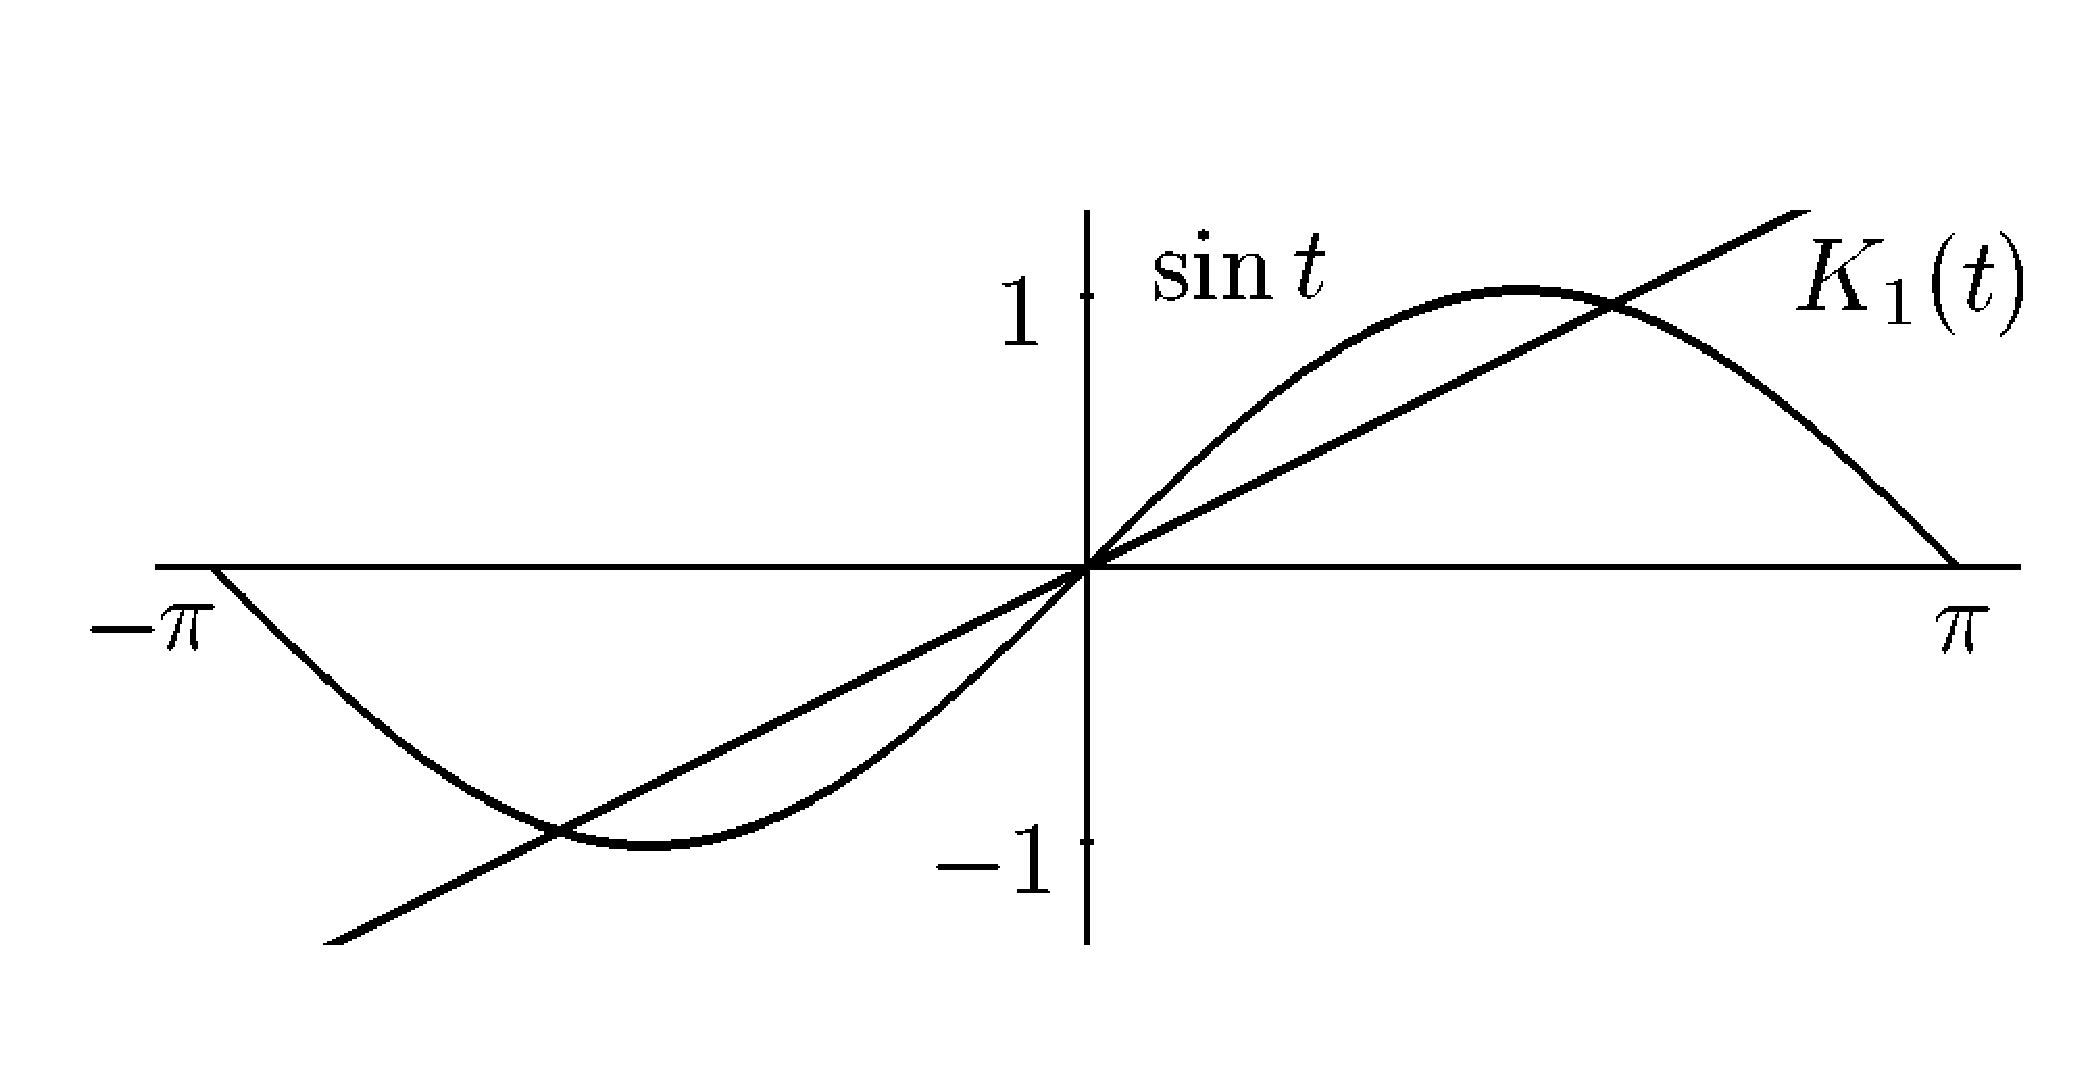
\includegraphics[width=0.5\textwidth]{pict/pict18-1.eps}
\end{center}
 \refstepcounter{ris}\label{r18-1}

 \centerline{Рис.~\theris}
\end{figure}





 \begin{lemma}\label{l18-2}
 Разность $R=K_r-U_{n-1}$ ядра $K_r$ и интерполяционного
 полинома
 $U_{n-1}$ обладает свойством
 $$
 \sign(K_r(t)-U_{n-1}(t))=\pm \sign \sin nt,\qquad t\in(-\pi,\pi),
 $$
  если число $r$ нечетное, и свойством
 $$
 \sign(K_r(t)-U_{n-1}(t))=\pm \sign \cos nt,\qquad t\in(-\pi,\pi),
 $$
  если число $r$ четное.
 \end{lemma}

Д\;о\;к\;а\;з\;а\;т\;е\;л\;ь\;с\;т\;в\;о\quad леммы~\ref{l18-2}.
Разность $R=K_r-U_{n-1}$ на $(-\pi,\pi)$ имеет $(2n-1)$ нулей при нечетном $r$ и
$2n$ нулей -- при четном $r.$ Для обоснования утверждений леммы достаточно
показать, что все эти нули простые и других нулей нет.

В свою очередь, для этого достаточно доказать, что при $r$ нечетном
для произвольного нечетного тригонометрического полинома $V_{n-1}$ порядка $n-1$ разность
$R=K_r-V_{n-1}$ имеет на $(-\pi,\pi)$ не более $(2n-1)$ нулей (с учетом их
кратности), а при четном $r$ и четном полиноме $V_{n-1}$
разность $R=K_r-V_{n-1}$  имеет на $(-\pi,\pi)$ не более
$2n$ нулей {(опять же с учетом их
кратности).} Докажем это утверждение  индукцией по $r\ge 1.$


1. Пусть $r=1.$ Покажем, что разность $R=K_1-V_{n-1}$ между ядром $K_1$ (оно в данном
случае нечетное) и нечетным тригонометрическим
  полиномом $V_{n-1}$ имеет на интервале $(-\pi,\pi)$ не более $(2n-1)$
  нулей (с учетом их кратности).
  Докажем этот факт от противного. Производная разности
 $$
 R'(t)=\frac{1}{2} -V_{n-1}'(t)=\frac{1}{2} -\sum\limits_{k=1}^{n-1}
 \alpha_k\cos kt,\qquad t\in (-\pi,\pi),
 $$
 есть (ненулевой) полином по  косинусам порядка $n-1$. Такой полином
 может иметь на $(-\pi,\pi)$
 не более $(2n-2)$ нулей. Если бы на $(-\pi,\pi)$ разность $R$ имела,
 по крайней мере,  $2n$
 нулей, то по теореме Ролля ее производная  $R'$ имела бы $(2n-1)$
 нулей, чего быть не может. Пришли к противоречию. Следовательно,
 $R=K_r-V_{n-1},$ действительно,
 имеет на $(-\pi,\pi)$ не более $(2n-1)$ нулей.

 2. Пусть $r=2.$ Ядро  $K_2$ и полином $V_{n-1}$  являются четными.
 Мы хотим  доказать, что разность
 $R=K_2-V_{n-1}$ имеет на $(-\pi,\pi)$
 не более $2n$ нулей.
 Имеем  $R'=K_2'(t)-V'_{n-1}$, где
 $V'_{n-1}$ есть  нечетный полином порядка $n-1$. Только что  мы уже доказали, что такая
 разность может иметь не более $(2n-1)$ нулей на $(-\pi,\pi).$
 Следовательно, $R$ может иметь не более $2n$ нулей.

 3. Докажем теперь, что если при  $r>1$ нужное свойство нулей  имеет место для номера $r-1,$ то оно имеет место и для номера $r.$    Пусть $r>1$ нечетное,
 $r=2s+1,$~ $s\ge 1.$
 Тогда $K_{2s+1}$ и $V_{n-1}$ нечетные и, следовательно  $K_{2s+1}$
 и $V_{n-1}$ обращаются в точках $\pm \pi$
 в нуль. Но тогда и разность  $R=K_{2s+1}-V_{n-1}$ также в этих точках обращается в нуль:
 $R(\pm \pi)=0.$
  Докажем, что число нулей $m$ разности  $R$ на $(-\pi,\pi)$ не превосходит
  $2n-1.$ Поскольку $R(\pm\pi)=0,$ то по теореме Ролля производная $R'$
   будет иметь  $m+1$ нуль на интервале $(-\pi,\pi).$ По  предположению же
   индукции производная  $R'=K_{r-1}-V'_{n-1}$
 имеет на $(-\pi,\pi)$ не более $2n$ нулей. Следовательно,  число нулей
 разности  $R=K_{2s+1}-V_{n-1}$ не превосходит числа $2n-1.$


 Если $r=2s$ четное, то $R'=K_{2s-1}-V'_{n-1}$ есть функция нечетная и по доказательству
  имеет не более $(2n-1)$ нулей. По теореме Ролля  разность $R$ имеет не более $2n$
 нулей. Лемма доказана.

 Теперь можно выписать наилучшее приближение ядра Бернулли {\eqref{f18-13}} тригонометрическими полиномами в
 среднем.

 \begin{teo}\label{t18-2}
 Полином $U_{n-1}$ порядка $n-1,$ интерполирующий ядро  $K_r$
 в нулях $\sin nx$, если число $r$ нечетное, и в нулях  $\cos nx$, если число $r$ четное,
 является полиномом наилучшего приближения для $K_r$ в пространстве $L;$ при этом
 \begin{equation}\label{f18-14}
 E_{n-1}(f)_L=\|K_r-U_{n-1}\|_L=\frac{M_r}{n^r}, %\eqno(14)
 \end{equation}
 где
 \begin{equation}\label{f18-15}
 M_r=\frac{4}{\pi}\sum\limits_{k=0}^{\infty}
 \frac{(-1)^{(r+1)k}}{(2k+1)^{r+1}}. %\eqno(15)
 \end{equation}
 \end{teo}




  Д\;о\;к\;а\;з\;а\;т\;е\;л\;ь\;с\;т\;в\;о\quad теоремы~\ref{t18-2}.
  Экстремальность полиномов $U_{n-1}$ была обоснована в предшествующих рассуждениях.
  Далее, применяя формулы~{$(\ref{f18-6}''),$ $(\ref{f18-7}'')$}, {{$(\ref{f18-5}'),$
  $(\ref{f18-5}'')$}} и разложение~{\eqref{f18-13},}  получаем
  $$
 E_{n-1}(f)_L=\left|\frac{1}{\pi}\int_{-\pi}^{\pi}K_r(t)\sign \sin nt\,dt\right|=  \frac{4}{\pi}\, \sum\limits_{k=0}^{\infty}
 \frac{1}{n^r(2k+1)^{r+1}},\qquad r - \mbox{нечетное},
  $$
  $$
 E_{n-1}(f)_L=\left|\frac{1}{\pi}\int_{-\pi}^{\pi}K_r(t)\sign \cos nt\,dt\right|= \frac{4}{\pi}\, \sum\limits_{k=0}^{\infty}
 \frac{(-1)^{k}}{n^r(2k+1)^{r+1}},\qquad r - \mbox{четное}.
 $$
 Теорема доказана.


\ \
